\documentclass{article}

\usepackage[biblatex, letter]{preamble}
\addbibresource{refs.bib}

\NewDocumentCommand{\evalat}{sO{\big}mm}{%
  \IfBooleanTF{#1}
   {\mleft. #3 \mright|_{#4}}
   {#3#2|_{#4}}%
}

\title{Modelling Surface Acoustic Wave Driven Thin Film Flows over Topography}
\author{Bhargav Samineni}
\date{\today}

\begin{document}
 
\maketitle  

\begin{abstract}
    Motivated by the acoustowetting phenomenon and its applications to the dynamic wetting 
    of objects by a coating liquid, we explore the influence of surface acoustic waves and gravity on the motion of a thin film
    flowing over a surface. We consider surfaces that may be both inclined and include topographical features like trenches, mounds, bumps, etc. 
    Using the lubrication approximation, we reduce the equations of motion for the film
    to a single nonlinear partial differential equation that describes the evolution of the film height relative to the 
    surface topography in time and space. 
\end{abstract}
  
%\dosecttoc
%\tableofcontents
 
\section{Introduction}
The motion of thin liquid films with fronts is a relatively
ubiquitous dynamic in nature that also has applications to a number of technical fields and processes. 
Particularly with respect to coating processes, the influence of other factors besides viscous and surface tension
forces (such as gravity \cite{diez2002computing} and electric fields \cite{veremieiev2012electrified}) has also been 
studied. Recent experiments have shown that high frequency surface acoustic waves may be a novel method 
for coating techniques, particularly between two liquids where one of the liquids is not influenced by the acoustic streaming, so in this report we study the affect of these acoustic waves on the dynamics 
of thin liquid films. Specifically, we approach the problem using the lubrication approximation to reduce the 
Navier-Stokes equations into a single nonlinear PDE and simplify the interactions between the two liquids
by considering the stationary one to be a topographical feature of our surface. Both the influence of surface acoustic
waves on the spreading of liquid films (see \cite{altshuler2016free}) and coating over topography with gravity as the primary driving have been previously 
studied (see \cite{kalliadasis2000steady,stillwagon1988topo,veremieiev2011gravity}), but to the best of our knowledge the 
intersection of these two interactions has not been studied. 

\section{Governing Equation} \label{sec:gov_eq}

\subsection{Lubrication Approximation}
As shown in \cite{kondic2003instabilities}, if the Reynold's number is sufficiently low, the inertial terms of the Navier-Stokes equations 
can be ignored. Thus, under the effects of gravity and SAW streaming forces the lubrication approximation gives
\begin{gather}
    \grad_2 p = \mu \frac{\partial^2 \vect{v}}{\partial z^2} + \rho g \sin\theta \vect{i} - J\cexpz\vect{i}
    \label{eq:pressure_grad}\\
    \pderiv{p}{z} = -\rho g \cos\theta - J\alpha_1 \cexpz
    \label{eq:pressure_z}
\end{gather}
where $J = \rho \lrp{1 + \alpha_1^2}A^2\omega^2k_i$,  $\grad_2 = \lrp{\partial_x, \partial_y}$, 
and $\vect{v} = \lrp{u, v}$. 

\subsection{Boundary Conditions}
\subsubsection{Laplace-Young Boundary Condition}
The Laplace-Young boundary condition states that at the interface $z = \func{\phi}{x, y, t}$, the pressure is given by 
$\func{p}{\phi} = -\gamma \kappa + p_0$, where $\kappa$ is the curvature of the boundary, $\gamma$ is the surface tension, and $p_0$ is the atmospheric pressure. 
Thus, integrating \cref{eq:pressure_z} gives 
\begin{align}
    \nonumber \int_{\phi}^{z} \pderiv{p}{z} \; dz &=  \int_{\phi}^{z} -\rho g \cos \theta - J\alpha_1 \cexpz \; dz\\
    \nonumber \func{p}{z} - \func{p}{\phi} &= -\lrp{z - \phi} \rho g \cos \theta - \frac{J}{2k_i} \lrp{\cexpz - \cexpp}\\
    \func{p}{z} &= -\lrp{z - \phi}\rho g \cos \theta - \frac{J}{2k_i} \lrp{\cexpz - \cexpp} -\gamma \kappa + p_0.  
    \label{eq:laplace_young}
\end{align}
If we define 
\begin{align}
    \func{P}{x, y, t} = \phi \rho g \cos\theta + \frac{J}{2k_i} \cexpp - \gamma\kappa, 
    \label{eq:cap_P}
\end{align}
this simplifies \cref{eq:laplace_young} to 
\begin{align*}
    \func{p}{z} = P - z\rho g \cos\theta - \frac{J}{2k_i}\cexpz + p_0
\end{align*}
which further gives 
\begin{align}
    \grad_2 p %= \grad_2 \lrp{P - z\rho g \cos\theta - \frac{J}{2k_i}\cexpz + p_0}
    = \grad_2 \lrp{P - \frac{J}{2k_i}\cexpz}
    = \grad P - J\cexpz \vect{i}
    \label{eq:grad2_p_expanded}
\end{align}

\subsubsection{Further Boundary Conditions}
Further boundary conditions include 
\begin{gather}
    \evalat{\vect{v}}{z = s\lrp{x,y}} = \vect{0} 
    \label{eq:bound_noslip}\\
    \evalat[\Big]{\pderiv{\vect{v}}{z}}{z = \phi\lrp{x,y,t}} = \vect{0} 
    \label{eq:bound_stress}
\end{gather}
where \cref{eq:bound_noslip} is a no-slip BC along the surface $z = \func{s}{x,y}$ and \cref{eq:bound_stress}
enforces vanishing shear stresses along the fluid-air boundary $z = \func{\phi}{x,y,t}$. 

\subsection{Film Equation}
\subsubsection{Velocity Vector Equation}
Under the Laplace-Young BC and \cref{eq:grad2_p_expanded}, \cref{eq:pressure_grad} simplifies into 
\begin{align}
    \grad P = \mu \frac{\partial^2 \vect{v}}{\partial z^2} + \rho g \sin\theta \vect{i}. 
    \label{eq:pressure_grad_new}
\end{align}
Integrating \cref{eq:pressure_grad_new} twice with respect to $z$ and utilizing  
\cref{eq:bound_noslip} and \cref{eq:bound_stress} gives
\begin{align}
    \nonumber \int_{s}^{z}\int_{z}^{\phi} \pderivtwo{\vect{v}}{z} \; dzdz &= \frac{1}{\mu}\int_{s}^{z}\int_{z}^{\phi} \lrp{\grad P - \rho g \sin\theta\vect{i}} \; dzdz \\
    \nonumber \int_{s}^{z} \lrp{\evalat[\Big]{\pderiv{\vect{v}}{z}}{z = \phi} - \pderiv{\vect{v}}{z}} \; dz &= \frac{1}{\mu} \lrp{\grad P - \rho g \sin\theta\vect{i}} \int_{s}^{z}\lrp{\phi - z} \; dz\\
    \nonumber \int_{s}^{z} \pderiv{\vect{v}}{z} \; dz &= \frac{1}{\mu} \lrp{\grad P - \rho g \sin\theta\vect{i}} \int_{s}^{z} \lrp{z - \phi} \; dz\\
    \nonumber \vect{v} - \evalat{\vect{v}}{z = s} &= \frac{1}{\mu} \lrp{\grad P - \rho g \sin\theta\vect{i}}  \lrp{\frac{z^2}{2} - \phi z} \Bigg|_{s}^z\\
    \vect{v} &=\frac{1}{\mu} \lrp{\grad P - \rho g \sin\theta\vect{i}} \lrp{\frac{z^2}{2} - \phi z - \frac{s^2}{2} + \phi s}. 
    \label{eq:vel_vectv}
\end{align}

\subsubsection{Depth Averaged Velocity}
Averaging over the height removes the $z$ dependence of $\vect{v} = \lrp{u, v}$ and gives the equation 
\begin{align*}
    \bar{\vect{v}} = \frac{1}{h} \int_{s}^{\phi} \vect{v} \; dz.
    %\label{eq:vectv_bar_int}
\end{align*}
Solving this integral then gives 
\begin{align}
    \nonumber \bar{\vect{v}} &= \frac{1}{h} \int_{s}^{\phi} \frac{1}{\mu} \lrp{\grad P - \rho g \sin\theta\vect{i}} \lrp{\frac{z^2}{2} - \phi z - \frac{s^2}{2} + \phi s}  \; dz\\
    \nonumber &= \frac{1}{\mu h} \lrp{\grad P - \rho g \sin\theta\vect{i}} \lrp{\frac{z^3}{6} - \frac{\phi z^2}{2} - z\lrp{\frac{s^2}{2} - \phi s}} \Bigg|_{s}^{\phi}\\
    \nonumber &= \frac{1}{\mu h} \lrp{\grad P - \rho g \sin\theta\vect{i}} \lrp{-\frac{\phi^3}{3} + \phi^2s - \phi s^2 + \frac{s^3}{3}}\\
    \nonumber &=  \frac{1}{\mu h} \lrp{\grad P - \rho g \sin\theta\vect{i}} \lrp{-\frac{(h+s)^3}{3} + (h+s)^2s - (h+s) s^2 + \frac{s^3}{3}}\\
    &= -\frac{h^2}{3\mu} \lrp{\grad P - \rho g \sin\theta\vect{i}}.
    \label{eq:uv_bar}
\end{align}

\subsubsection{Conservation of Mass}
The conservation of mass, when depth-averaged, gives 
\begin{align}
    \pderiv{h}{t} + \grad \cdot \lrp{h\bar{\vect{v}}} = 0
\end{align}
which results in 
\begin{align}
    \nonumber \pderiv{h}{t} &= \frac{1}{3\mu} \grad \cdot \lrb{h^3 \lrp{\grad P - \rho g \sin \theta \vect{i}}}\\
    &= \frac{1}{3\mu} \grad \cdot \lrb{h^3 \lrp{\rho g \cos\theta \grad \phi - \gamma\grad\kappa - \rho g \sin \theta \vect{i} + \frac{J}{2k_i}\grad \cexpp }}. 
\end{align}
Approximating the curvature $\kappa \approx \grad^2 \phi$ then gives 
\begin{align}
    \nonumber \pderiv{h}{t} &= \frac{1}{3\mu} \grad \cdot \lrb{h^3 \lrp{\rho g \cos\theta \grad \phi - \gamma\grad\grad^2\phi - \rho g \sin \theta \vect{i} + \frac{J}{2k_i}\grad \cexpp}}\\
    &= \frac{1}{3\mu} \lrb{ \grad \cdot \lrb{\rho g \cos \theta h^3 \grad \phi} - \grad \cdot \lrb{\gamma h^3 \grad\grad^2\phi} - \rho g \sin\theta \pderiv{h^3}{x} + \grad \cdot \lrb{\frac{J}{2k_i}h^3\grad \cexpp}}.
    \label{eq:thin_film_dim}
\end{align}

\subsection{Dimensionless Form}
Scale the in-plane coordinates and time by 
\begin{gather}
    \bar{x} = \frac{x}{x_c}, \quad \bar{y} = \frac{y}{x_c}, \quad \bar{z} = \frac{z}{h_c}, \quad \bar{t} = \frac{t}{t_c}. 
    \label{eq:coord_time_scales}
\end{gather}
where an overline denotes a non-dimensional quantity. From these scales, we get that  
\begin{gather*}
    k_i = \frac{\bar{k_i}}{x_c}, \quad \omega = \frac{\bar{\omega}}{t_c}, \quad A = \bar{A}h_c
\end{gather*}
and thus that 
\begin{align}
    J = \rho \lrp{1 + \alpha_1^2}  \bar{A}^2 h_c^2 \frac{\bar{\omega}^2 \bar{k_i}}{t_c^2 x_c} = \frac{\rho \eta h_c^2}{t_c^2 x_c}
    \label{eq:J_nondim}
\end{align}
where $\eta = \lrp{1 + \alpha_1^2}  \bar{A}^2 \bar{\omega}^2 \bar{k_i}$ is non-dimensional. Substituting the scales in 
\cref{eq:coord_time_scales} and \cref{eq:J_nondim} into \cref{eq:thin_film_dim} and removing any bars gives 
\begin{multline}
    \frac{h_c}{t_c} \pderiv{h}{t} = \frac{1}{3\mu} \lrb{
        \frac{h_c^4}{x_c^2} \rho g \cos \theta \grad \cdot \lrb{h^3\grad\phi} - 
        \frac{\gamma h_c^4}{x_c^4} \grad \cdot \lrb{h^3 \grad \grad^2 \phi} - 
        \frac{h_c^3}{x_c} \rho g \sin\theta \pderiv{h^3}{x}
    }\\
    + \frac{1}{3\mu} \lrb{ 
        \frac{\eta \rho h_c^5}{2k_i t_c^2 x_c^2} \grad \cdot \lrb{h^3 \grad e^{2k_i \lrp{x + \alpha_1 \phi \lrp{h_c/x_c}}}}
    }.
    \label{eq:nondim_first}
\end{multline}
By virtue of the fact that we are dealing with a thin film, $h_c \ll x_c$. Additionally, by definition
$\alpha_1 = -i \alpha$ where 
\begin{equation*}
    \alpha = \lrp{1 - \lrp{V_r/V_w}^2}^{1/2}
\end{equation*}
with $V_r$ and $V_w$ being the velocity of the SAW in the solid substrate and fluid, respectively. Since 
$V_r > V_w$
\begin{equation*}
    \alpha = i \lrp{\lrp{V_r/V_w}^2 - 1}^{1/2} \quad \rightarrow \quad \alpha_1 = \lrp{\lrp{V_r/V_w}^2 - 1}^{1/2}
\end{equation*}
which is real and $\bigo{1}$. Thus, we can ignore any component of the exponent 
that is multiplied by $\alpha_1$ and $h_c / x_c$, which simplifies \cref{eq:nondim_first} to 
\begin{align}
    \nonumber \frac{h_c}{t_c} \pderiv{h}{t} &= \frac{1}{3\mu} \lrb{
        \frac{h_c^4}{x_c^2} \rho g \cos \theta \grad \cdot \lrb{h^3\grad\phi} - 
        \frac{\gamma h_c^4}{x_c^4} \grad \cdot \lrb{h^3 \grad \grad^2 \phi} - 
        \frac{h_c^3}{x_c} \rho g \sin\theta \pderiv{h^3}{x} + 
        \frac{\eta h_c^5}{2k_i t_c^2 x_c^2} \grad \cdot \lrb{h^3 \grad e^{2k_i x}}
        %\frac{\eta h_c^5}{t_c^2 x_c^2} \pderiv{}{x} \lrb{h^3 \grad e^{2k_i x}}. 
    }\\
    \nonumber &= \frac{\gamma h_c^4}{3\mu x_c^4} \lrb{
        \frac{x_c^2 \rho g}{\gamma} \cos \theta \grad \cdot \lrb{h^3\grad\phi} - 
        \grad \cdot \lrb{h^3 \grad \grad^2 \phi} - 
        \frac{x_c^3}{\gamma h_c} \sin\theta \pderiv{h^3}{x} + 
        \frac{\eta \rho x_c^2 h_c}{\gamma t_c^2} \pderiv{}{x} \lrb{h^3 e^{2k_i x}}
    }\\
    \pderiv{h}{t} &= \frac{\gamma h_c^3}{3\mu x_c^4 t_c} \lrb{
        \frac{x_c^2 \rho g}{\gamma} \cos \theta \grad \cdot \lrb{h^3\grad\phi} - 
        \grad \cdot \lrb{h^3 \grad \grad^2 \phi} - 
        \frac{x_c^3}{\gamma h_c} \sin\theta \pderiv{h^3}{x} + 
        \frac{\eta \rho x_c^2 h_c}{\gamma t_c^2} \pderiv{}{x} \lrb{h^3 e^{2k_i x}}
    }.
    \label{eq:nondim_sec}
\end{align}
Choose $x_c$ and $t_c$ such that 
\begin{align}
    x_c = \lrp{\frac{\gamma h_c}{\rho g}}^{1/3}, \quad t_c = \frac{3\mu x_c}{h_c^2 \rho g}.
    \label{eq:x_and_t_scales}
\end{align}
Substituting these scales into \cref{eq:nondim_sec} yields
\begin{align}
    \pderiv{h}{t} = \lrp{\frac{h_c^2 \rho g}{\gamma}}^{1/3} \cos\theta \grad \cdot \lrb{ h^3 \grad \phi } - 
    \grad \cdot \lrb{h^3 \grad\grad^2\phi } - 
    \sin\theta \pderiv{h^3}{x} + 
    \frac{\eta \rho x_c^2 h_c}{\gamma t_c^2} \pderiv{}{x} \lrb{h^3 e^{2k_i x}}.
    \label{eq:nondim_third}
\end{align}  
The velocity scale is chosen naturally as $U = x_c/t_c = h_c^2\rho g/3\mu$,
which allows us to additionally define the capillary number $\mathrm{Ca} = \mu U / \gamma = h_c^2\rho g/3\gamma$
and Weber number $\mathrm{We} = \rho U^2 h_c / \gamma = \rho x_c^2 h_c / \gamma t_c^2$, both of which
are non-dimensional quantities. Hence, 
\cref{eq:nondim_third} simplifies to 
\begin{align}
    \pderiv{h}{t} = \lrp{3\mathrm{Ca}}^{1/3} \cos\theta \grad \cdot \lrb{ h^3 \grad \phi } - 
    \grad \cdot \lrb{h^3 \grad\grad^2\phi } - 
    \sin\theta \pderiv{h^3}{x} + 
    \eta \mathrm{We} \pderiv{}{x} \lrb{h^3 e^{2k_i x}}.
    \label{eq:nondim_fourth}
\end{align}  
If we further define 
\begin{equation*}
    D = \lrp{3\mathrm{Ca}}^{1/3}, \quad C = \eta \mathrm{We}
\end{equation*}
then we get a final equation 
\begin{align}
    \pderiv{h}{t} = D \cos\theta \grad \cdot \lrb{ h^3 \grad \phi } - 
    \grad \cdot \lrb{h^3 \grad\grad^2\phi } - 
    \sin\theta \pderiv{h^3}{x} + 
    C \pderiv{}{x} \lrb{h^3 e^{2k_i x}}.
    \label{eq:nondim_final}
\end{align}  
 
\section{Method of Solution} \label{sec:method_of_sol}
\subsection{Spatial Discretization}
If we define the domain of interest as $\lrb{0, L_x}$, we can discretize the 
domain into points $x_j = j\Delta x$ for $j = 0, \ldots, N_x$ where 
$\Delta x = L_x / N_x$ and $N_x$ is the number of grid points excluding the origin. 
If we further define $\func{h_j}{t} = \func{h}{x_j, t}$, we can discretize 
\cref{eq:two_dim_final} into a system of ordinary differential equations of the form 
\begin{equation}
    \deriv{h_j}{t} = f_j = \mathrm{Bo}\cos \beta f_j^{(1)} - f_j^{(2)} -  \frac{\mathrm{Bo}}{\varepsilon} \sin \beta f_j^{(3)} +  
    \frac{k_i \lrp{1 + \alpha_1^2} \mathrm{We_{ac}}}{\varepsilon} f_j^{(4)}, \quad j = 0, \ldots, N_x
    \label{eq:ode_sys}
\end{equation}
where $f_j^{(k)}$ is the discretization of the $k$-th term in
the right-hand side of \cref{eq:two_dim_final}. Because the governing equation 
contains high order derivatives, the discretization used for certain components 
needs special attention in order to not lead to a large computational stencil.

\subsubsection{Fourth-Order Term}
Following the method outlined in \cite{kondic2003instabilities}, discretizing the fourth order term (i.e.\! $f_j^{(2)}$) can be done by a combination
of forward and backward differences. If we define 
\begin{align*}
    h_{x, j} = \frac{h_{j+1} - h_j}{\Delta x} \quad \quad \quad h_{\overline{x}, j} = \frac{h_{j} - h_{j-1}}{\Delta x}
\end{align*}
as the forward and backward differences, respectively, then a possible discretization is 
\begin{equation}
    f_j^{\lrp{2}} = \lrp{\func{a}{h_{i-1}, h_i} \phi_{\overline{x}x\overline{x}}}_{x}
    \label{eq:f2_disc}
\end{equation}
where $\func{a}{j_1, j_2} = \frac{1}{2} \lrp{{j_1}^3 + {j_2}^3}$. This discretization leads to a 
second order approximation that has a five point stencil, which is better than the seven point stencil
that would result from using a central differencing scheme. 

\subsubsection{Lower Order Terms}


\section{Numerical Simulations} \label{sec:results}
While we have developed equations to model the influence of both SAWs and gravity on the 
motion of thin films, we are primarily concerned with the case where the SAW is the primary driving
force. Hence, for all the simulations shown in this section we use $\beta = 0$. We also use the 
physical characteristics shown in \cref{tab:params}, a precursor film height of $b = 0.01$, as well as a drop initial condition for all the simulations. 
 
\begin{table}[hb]
    \centering
    \begin{tabular}{|lll|}
        \hline
        \multicolumn{3}{|c|}{Parameter Values}                                                                                    \\ \hline
        \multicolumn{1}{|l|}{Symbol}             & \multicolumn{1}{l|}{Physical Meaning}                & Quantitative Value          \\ \hline
        \multicolumn{1}{|l|}{$\rho$}             & \multicolumn{1}{l|}{Density of Oil}                  & 900 $\lrb{\frac{Kg}{m^3}}$  \\
        \multicolumn{1}{|l|}{$g$}                & \multicolumn{1}{l|}{Gravity}                         & 9.8 $\lrb{\frac{m}{s^2}}$   \\
        \multicolumn{1}{|l|}{$\mu$}              & \multicolumn{1}{l|}{Dynamic Viscosity of Oil}        & 0.45 $\lrb{\frac{Kg}{ms}}$                \\
        \multicolumn{1}{|l|}{$\gamma$}           & \multicolumn{1}{l|}{Surface Tension}                 & $20 \times 10^{-3} \lrb{\frac{Kg}{s^2}}$  \\
        \multicolumn{1}{|l|}{$A$}                & \multicolumn{1}{l|}{Amplitude of SAW}                & $8 \times 10^{-10} \lrb{m}$ \\
        \multicolumn{1}{|l|}{$\omega$}           & \multicolumn{1}{l|}{Angular Frequency of SAW}        & $2\pi \times 20 \times 10^6 \lrb{s^{-1}}$ \\
        \multicolumn{1}{|l|}{$\alpha_1$}         & \multicolumn{1}{l|}{Geometric Constant}              & 2.386                       \\
        \multicolumn{1}{|l|}{$k_i^{\text{oil}}$} & \multicolumn{1}{l|}{Attenuation Coefficient in Oil}  & $-1000 \lrb{m^{-1}}$                      \\
        \multicolumn{1}{|l|}{$k_i^{\text{air}}$} & \multicolumn{1}{l|}{Attenuation Coefficient in Air}  & $-1 \lrb{m^{-1}}$                         \\
        \multicolumn{1}{|l|}{$\lambda$}          & \multicolumn{1}{l|}{Steepness of Attenuation Coefficient Change}  & $2 \times 10^{-3} \lrb{m}$                         \\
        \multicolumn{1}{|l|}{$h_c$}              & \multicolumn{1}{l|}{Characteristic Film Thickness}   & $200 \times 10^{−6} \lrb{m}$              \\
        \multicolumn{1}{|l|}{$x_c$}              & \multicolumn{1}{l|}{Characteristic Length Scale}     & $10^{−3} \lrb{m}$           \\
        \multicolumn{1}{|l|}{$t_c$}              & \multicolumn{1}{l|}{Characteristic Time Scale}       & $ .84375 \lrb{s}$           \\
        \multicolumn{1}{|l|}{$\varepsilon$}      & \multicolumn{1}{l|}{Small Parameter}                 & $0.2$                       \\
        \multicolumn{1}{|l|}{$\mathrm{Bo}$}      & \multicolumn{1}{l|}{Bond Number}                     & $0.441$                     \\
        \multicolumn{1}{|l|}{$\mathrm{We_{ac}}$} & \multicolumn{1}{l|}{Acoustic Weber Number}           & $0.45479$                   \\ \hline
    \end{tabular}
    \caption{Physical parameters and their values used in our simulations}
    \label{tab:params}
\end{table}

\subsection{Flat Topography}
In this simulation we consider the scenario where we have a flat topography (i.e. $\func{s}{x} = 0$). This 
corresponds to a single initial drop being moved by SAW forcing with no other liquids in its path. We see in 
\cref{fig:flat_profile} that the initial oil drop moves from left to right and spreads out as it does so, which 
is consistent with experimental observations. We also note the formation of a capillary ridge near the contact line between the oil 
and the surface, which is also consistent with experimental observations. 

\begin{figure}[ht]
    \centering
    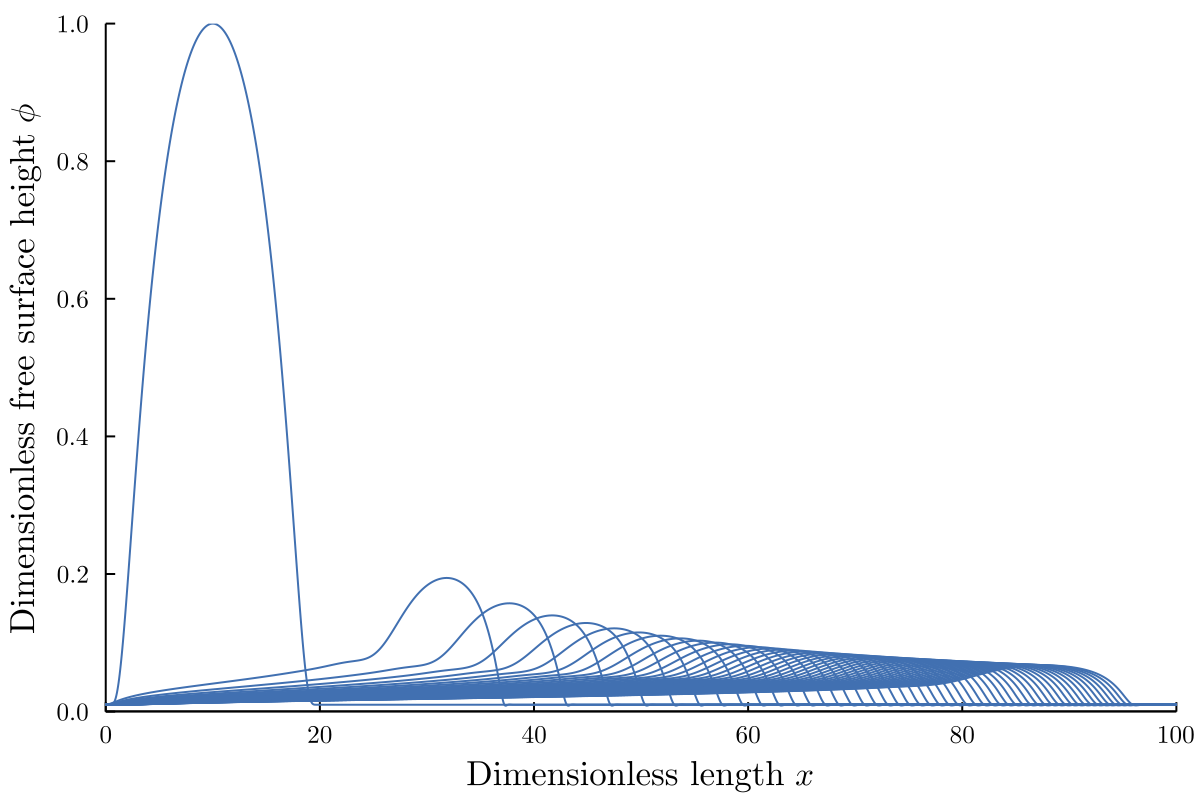
\includegraphics[scale=0.3]{images/flat/plt_notitle.png}
    \caption{Fluid profile on a flat topography plotted every $\Delta t = 10000$ dimensionless time units}
    \label{fig:flat_profile}
\end{figure}

\subsection{Bump Topography}
In the following simulations we consider the scenario where we have a bump topography (see \cref{sec:topography} in the appendix for 
a general bump equation). This corresponds to a single initial drop being moved by SAW forcing with 
another liquid in its path being modelled by the stationary bump.  
In the case where the maximum height of our bump is small, we find that the initial oil drop is able to 
clear the bump and spread over the entire domain as shown in \cref{fig:bump05_profile}. 
However, in the case where the maximum height is large, we find that the initial oil drop is not able to 
clear the bump and gets stuck on it as shown in \cref{fig:bump10_profile}. 
This behavior showcases an inherent limitation of our model in that modelling another liquid as a 
stationary feature of the surface topography does not allow the \textquote{leaky} effects of the surface acoustic wave
to be transferred to the moving liquid as it flows over the bump. Essentially, the effect of acoustic driving 
is lost over the bump region as we consider it to be solid instead of liquid, which is not in acceptance with experimental observations. 


\section{Conclusion} \label{sec:conclusion}
The presented results show that a reasonably accurate model can be developed for simulating the movement of thin 
film flows over topography when driven primarily by SAWs. We first develop a governing nonlinear PDE by simplifying the 
incompressible Navier-Stokes equations for the problem using the lubrication approximation, with a further simplification 
to reduce our equation to two spatial dimensions instead of three. We then solve the PDE over a domain of interest by discretizing 
into a system of ODEs, which is then solved using an implicit time stepping scheme. However, a limitation of our model is that 
it does not realistically model the interactions between a flowing and stationary liquid as the assumption that the stationary liquid can be 
modelled as a feature of the surface topography does not take into the account of leakiness of SAWs in liquids. 

\begin{figure}[h]
    \centering
    \begin{subfigure}[b]{0.5\textwidth}
        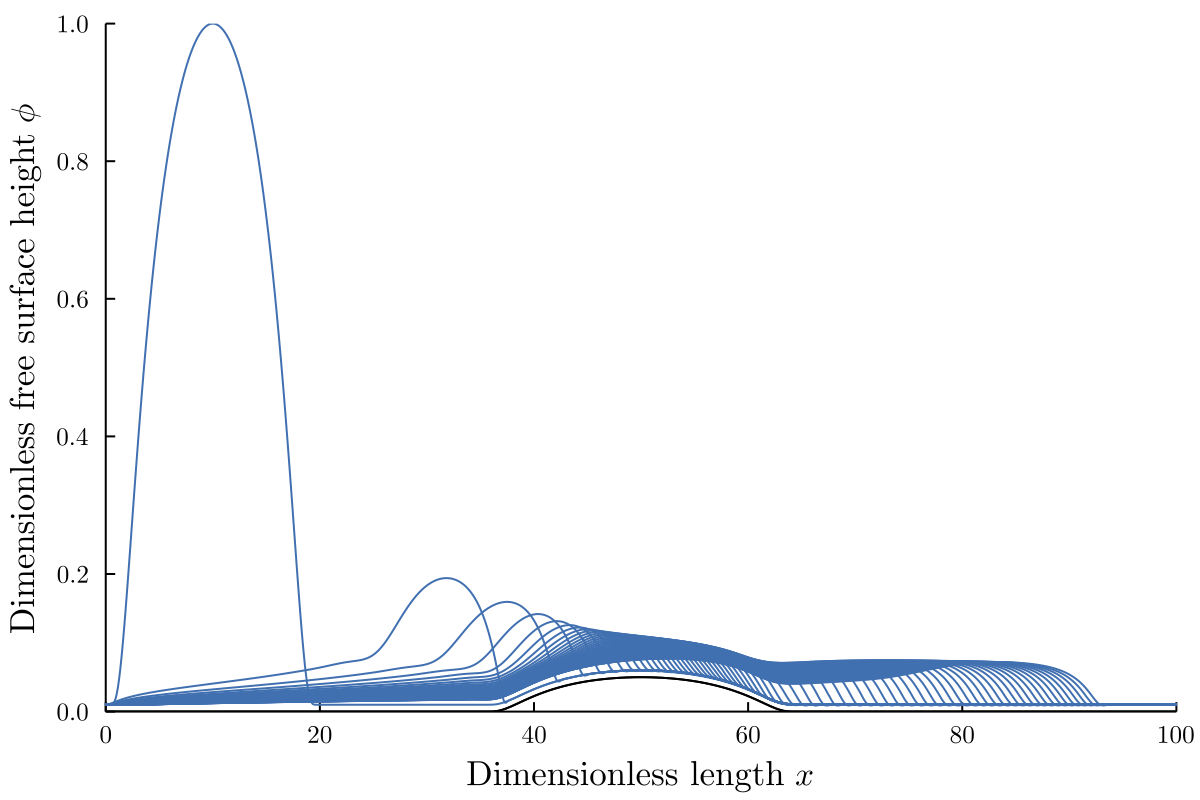
\includegraphics[width=\textwidth]{images/bump_05/plt_notitle.png}
        \caption{Small bump}
        \label{fig:bump05_profile}
    \end{subfigure}%
    \begin{subfigure}[b]{0.5\textwidth}
        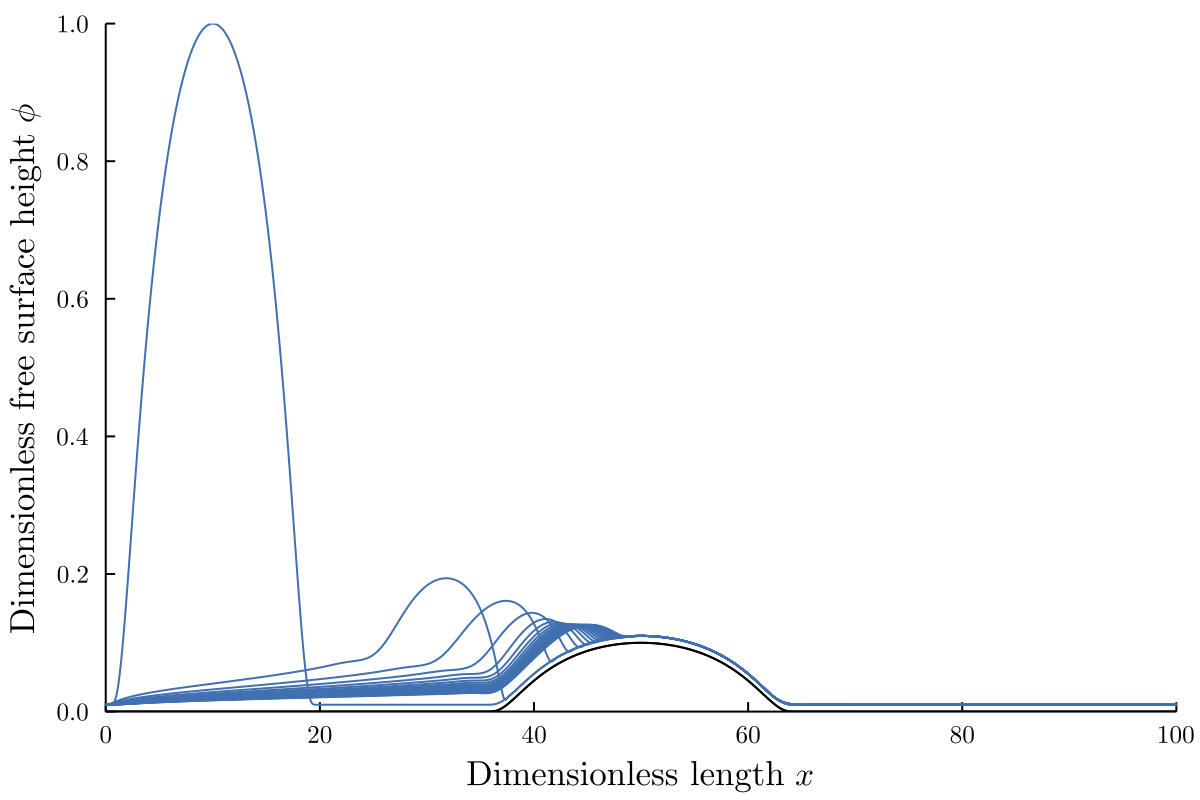
\includegraphics[width=\textwidth]{images/bump_10_shorter/plt_notitle.png}
        \caption{Tall bump}
        \label{fig:bump10_profile}
    \end{subfigure}
    \caption{Fluid profile on bump topographies plotted every $\Delta t = 10000$ dimensionless time units}
    \label{fig:bump_profiles}
\end{figure}
 
\newpage
\begin{appendices}
    If we define 
\begin{equation*}
    \func{a}{j_1, j_2} = \frac{1}{2} \lrp{\lrp{\func{h}{j_1, t}}^3 + \lrp{\func{h}{j_2, t}}^3} = \frac{1}{2} \lrp{h_{j_1}^3 + h_{j_2}^3}
\end{equation*}
as an approximation to $h^3$, then 
\begin{gather*}
\begin{aligned}
    f_i^{(1)} &= \frac{1}{\Delta x^2} \lrp{\func{a}{j-1, j}\lrp{\phi_{j-1} - \phi_{j})} + \func{a}{j, j+1}\lrp{\phi_{j+1} - \phi_{j}}}\\
    &= \frac{1}{2\Delta x^2} \lrp{\lrp{h_{j-1}^3 + h_{j}^3}\lrp{\phi_{j-1} - \phi_{j})} + \lrp{h_{j}^3 + h_{j+1}^3}\lrp{\phi_{j+1} - \phi_{j}}}
\end{aligned}\\
\begin{aligned}
    f_i^{(2)} &= \frac{1}{\Delta x^4} \lrp{\func{a}{j-1, j}\lrp{\phi_{j-2} - 3\phi_{j-1} + 3\phi_{j} - \phi_{j+1}} + \func{a}{j, j+1}\lrp{-\phi_{j-1} + 3\phi_{j} - 3\phi_{j+1} + \phi_{j+2}}}\\
    &= \frac{1}{2\Delta x^4} \lrp{\lrp{h_{j-1}^3 + h_{j}^3} \lrp{\phi_{j-2} - 3\phi_{j-1} + 3\phi_{j} - \phi_{j+1}} + \lrp{h_{j}^3 + h_{j+1}^3} \lrp{-\phi_{j-1} + 3\phi_{j} - 3\phi_{j+1} + \phi_{j+2}}}
\end{aligned}\\
\begin{aligned}
    f_i^{(3)} = \frac{1}{2\Delta x} \lrp{h_{j+1}^3 - h_{j-1}^3}
\end{aligned}\\
\begin{aligned}
    f_i^{(4)} = \frac{1}{2\Delta x} \lrp{h_{j+1}^3 e^{2k_ix_{j+1}} - h_{j-1}^3 e^{2k_ix_{j-1}}}
\end{aligned}
\end{gather*}

\end{appendices}

\newpage
\printbibliography

\end{document} 